\documentclass[12pt,a4paper,notitlepage,twoside]{article}
\usepackage[utf8]{inputenc}
\usepackage{graphicx}
\usepackage{subcaption}
\usepackage{float}
\usepackage{listings}
\author{Robert James}
\begin{document}
\begin{Large}
\begin{center}
$02/03/15$ - $17/03/15$
\end{center}
\end{Large}

\section{Dissertation}

\begin{lstlisting}[breaklines]

\end{lstlisting}


\section{Code}

\begin{lstlisting}[breaklines]

\end{lstlisting}

\section{Data and Results}
\subsection{Metropolis Thermodynamic Quantities}

The Specific Heat Capacity was calculated using
\begin{equation}
C_V = \frac{1}{T^2} \left[ <E^2> - <E>^2 \right]
\end{equation}

The Magnetic Susceptibility was calculated using
\begin{equation}
\chi = \frac{1}{T} \left[ <M^2> - <M>^2 \right]
\end{equation}


\begin{figure}[H]
\centering
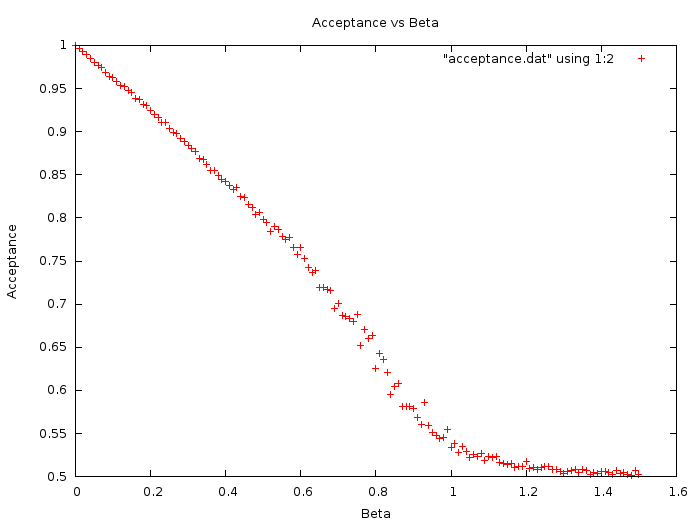
\includegraphics[width=0.4\textwidth]{q2d20/acceptance.png}
\caption{Acceptance for $q=2$ on a $20*20$ grid}
\end{figure}

\begin{figure}[H]
\centering
	\begin{subfigure}[b]{0.45\textwidth}
		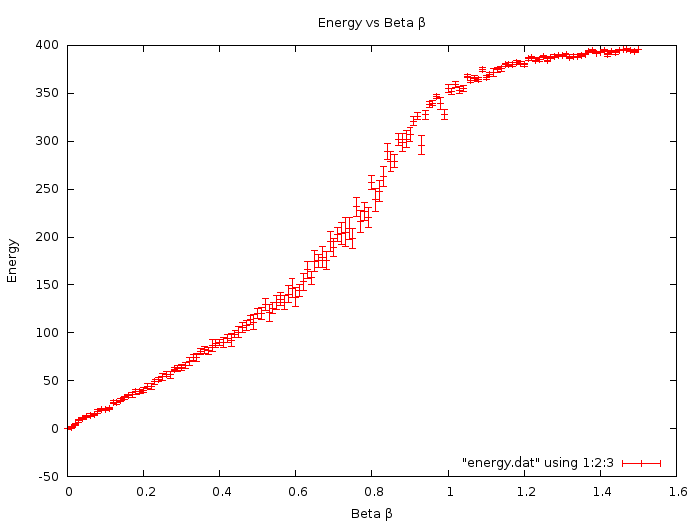
\includegraphics[width=\textwidth]{q2d20/energy.png}	
		\caption{Energy per Lattice Site with Errors}
	\end{subfigure}
	%
	\begin{subfigure}[b]{0.45\textwidth}
		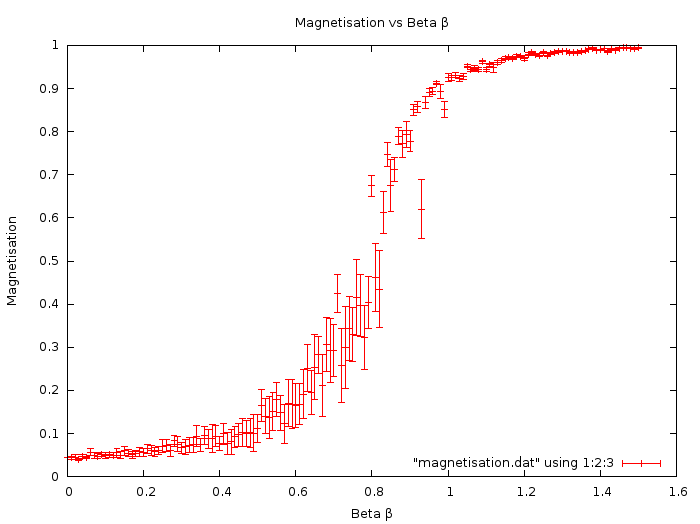
\includegraphics[width=\textwidth]{q2d20/magnetisation.png}
		\caption{Magnetisation per Lattice Site with Errors}
	\end{subfigure}
	%
\end{figure}

\begin{figure}[H]
\centering
	\begin{subfigure}[b]{0.45\textwidth}
		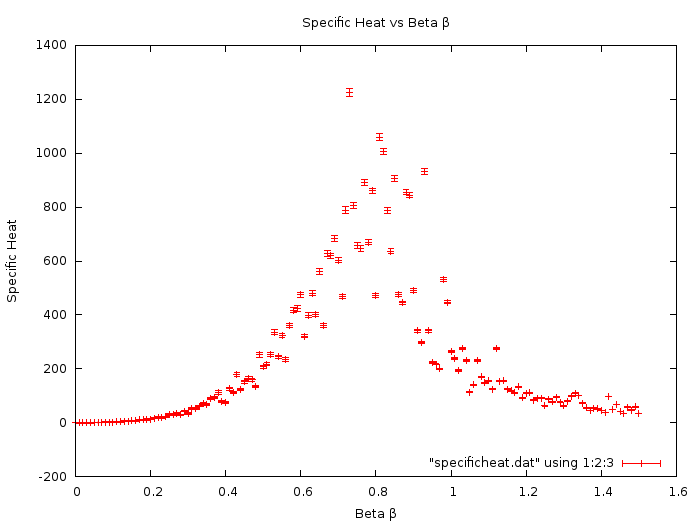
\includegraphics[width=\textwidth]{q2d20/specificheat.png}	
		\caption{Specific Heat of the System with Errors}
	\end{subfigure}
	%
	\begin{subfigure}[b]{0.45\textwidth}
		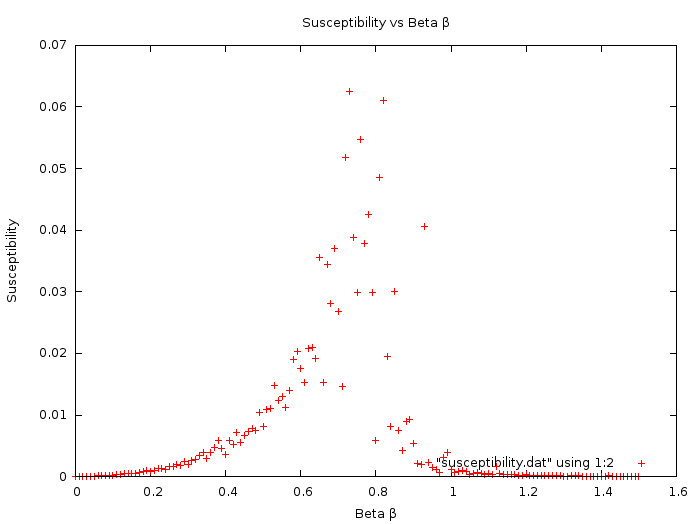
\includegraphics[width=\textwidth]{q2d20/susceptibility.png}
		\caption{Magnetic Susceptibility without errors}
	\end{subfigure}
	%
\end{figure}

Because the Error of the Magnetic Susceptibility becomes significantly larger than the data itself around $\beta_c$ it was not shown in this plot as to show the behaviour.

Behaviour is as expected when coupling is $J = 1/2$ to match the Ising Model. However when changing to the Antiferromagnetic case $J=-0.5$ the simulation becomes erratic.
Further investigation will be required to identify the source of the problem.

\subsection{an Convergence}

\begin{figure}[H]
\centering
\begin{subfigure}[b]{0.45\textwidth}
	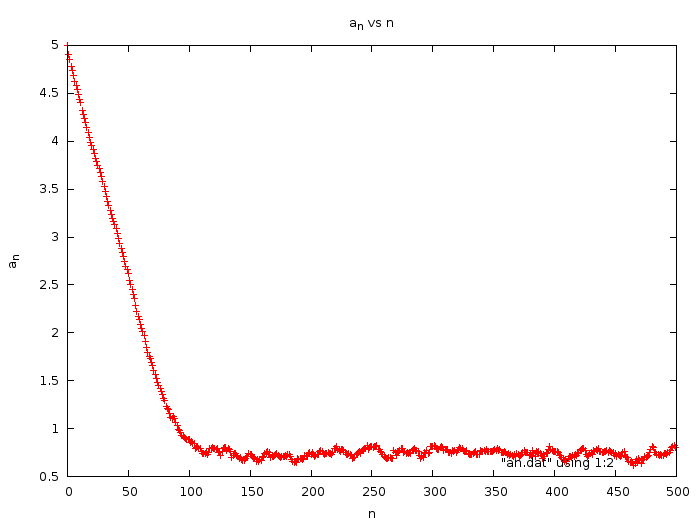
\includegraphics[width=0.9\textwidth]{q2d20/anconvergence.png}
	\caption{$q=2$}
\end{subfigure}
	%
\begin{subfigure}[b]{0.45\textwidth}
	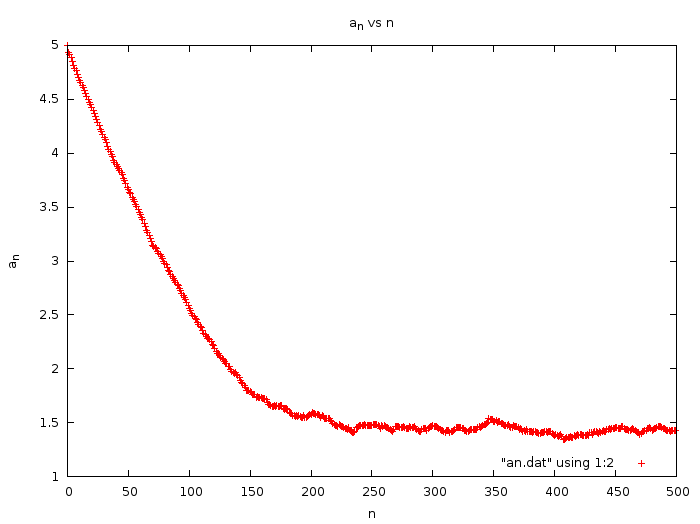
\includegraphics[width=0.9\textwidth]{q4d20/anconvergence.png}
	\caption{$q=4$}
\end{subfigure}

\begin{subfigure}[b]{0.45\textwidth}
	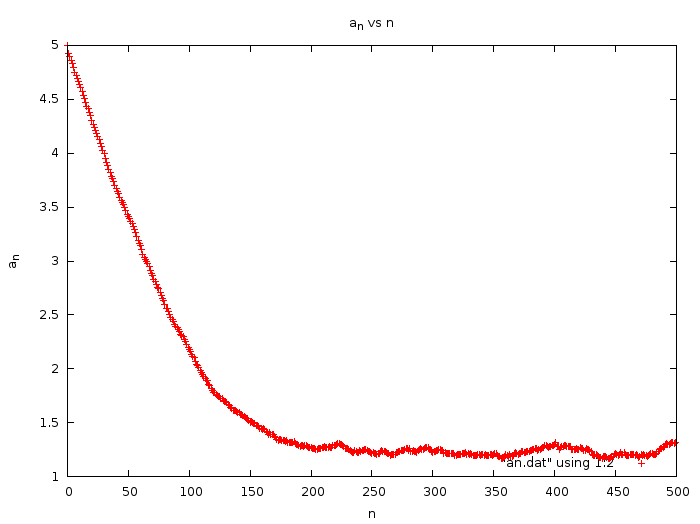
\includegraphics[width=0.9\textwidth]{q10d20/anconvergence.png}
	\caption{$q=10$}
\end{subfigure}
\caption{Target Energy: $-100.0$, Energy Band Width: $15.0$}
\end{figure}

Taking the energies calculated from the Metropolis at various $\beta$ and using those as a target to drive the configuration into to calculate $a_n$. I intend to prove that the two different values are indeed compatible.

\end{document}